\documentclass[border=12pt]{standalone}
\usepackage[utf8]{inputenc}
\usepackage[utf8]{vietnam}
\usepackage{amsmath,amsfonts,amssymb}
\usepackage{tikz}
\usepackage{flowchart}
\usetikzlibrary{arrows,decorations.markings,calc,fadings,decorations.pathreplacing,patterns,decorations.pathmorphing,positioning}

\begin{document}
    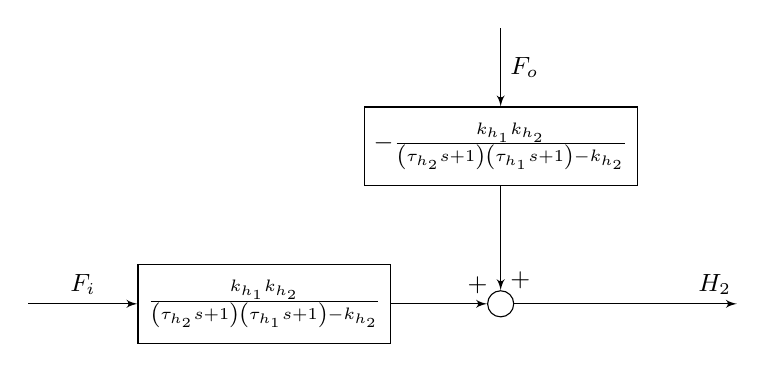
\begin{tikzpicture}[>=latex',font={\small}]
        \def\smbwd{2cm}
        \coordinate (f_i) at (-3, 0);
        \coordinate (f_o) at (3, 3.5);
        \coordinate (h_2) at (6, 0);
        \node (hamtruyen_fi) at (0, 0) [draw, process, minimum width=\smbwd, minimum height=1cm] {$\frac{k_{h_1} k_{h_2}}{\left({\tau_{h_2}s + 1}\right)\left({\tau_{h_1} s + 1}\right) - k_{h_2}}$};
        \node (hamtruyen_fo) at (3, 2) [draw, process, minimum width=\smbwd, minimum height=1cm] {$-\frac{k_{h_1} k_{h_2}}{\left({\tau_{h_2}s + 1}\right)\left({\tau_{h_1} s + 1}\right) - k_{h_2}}$};

        \node (sum_h2) at (3, 0) [circle, draw] {}; \coordinate (label_h) at (14, 0);

        \draw[->] (f_i) -- node[above]{$F_i$} (hamtruyen_fi);
        \draw[->] (f_o) -- node[right]{$F_o$} (hamtruyen_fo);
        \draw[->] (hamtruyen_fi) -- node[above,pos=0.9]{$+$} (sum_h2);
        \draw[->] (hamtruyen_fo) -- node[right,pos=0.9]{$+$} (sum_h2);
        \draw[->] (sum_h2) -- node[above,pos=0.9]{$H_2$} (h_2);
    \end{tikzpicture}

\end{document}
